\subsection{Quad-Tree}

Nous avons implémenté une autre manière de considérer les formes lors du packing en utilisant une structure de donnée particulière : les \texttt{quadtrees}.

\subsubsection{Principe général}

Prenons la bounding box d'un multi polygone. On le représente par une matrice de 0 et de 1 (bitmap). L'algorithme de création du quadtree consiste en subdivisions successives de la bounding box en zones. On délimite la bounding box de départ en 4 parties de tailles égales, puis on délimite ces zones en 4 parties récursivement, jusqu'à arrivée à un stade terminal.

A chaque itération, on regarde si une partie du multi polygone est contenue dans la zone en cours. Si non, on considère la zone comme "blanche" (0) et la récursivité se termine sur cette zone. Si le multi polygone recouvre intégralement la zone en cours, on considère cette dernière comme "noire" (1) et la récursivité se termine également. Le stade terminal peut également être une zone de taille atomique (pixel), une zone de précision voulue. 

Si le multi polygone est en partie dans la zone en cours, il s'agit d'une zone dite "grise", c'est-à-dire que la précision de la zone n'est pas suffisante pour décrire suffisamment le multi polygone sous forme de quadtree. Dans ce cas-ci, la subdivision récursive a lieu. Quelques itérations sont représentées en figure ~\ref{fig:quadtreeprinciple}.

\begin{figure}[H]
\centering
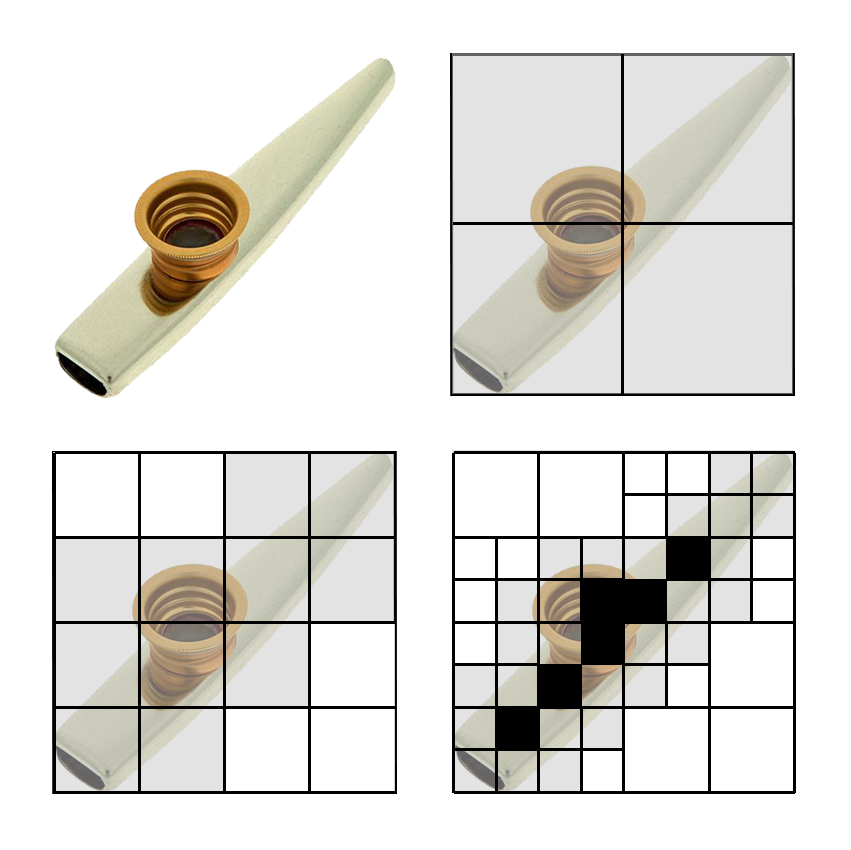
\includegraphics[scale=0.5]{img/quadtreeprinciple.png}
\caption{Principe du quadtree, itérations 0 à 3.}
    \label{fig:quadtreeprinciple}
\end{figure}

\subsubsection{Représentation}

Un Quadtree est une classe de même nom contenant plusieurs InnerQuadTree avec plusieurs informations sur ces derniers pour les utiliser par la suite. Plus clairement, on a choisi de précalculer pour un même multi polygone plusieurs quadtrees pour un ensemble de rotations possibles (30 degrés par défaut, donc 12 quadtrees précalculés). La classe Quadtree les garde en mémoire, ainsi que les offsets nécessaires (pour gérer la différence de point d'origine entre un multi polygone (au centre) et un quadtree(en haut à gauche)), les centres de gravité de chaque rotation (centroids) et d'autres informations (précision de l'approximation etc).\\


Les InnerQuadTrees s'occupent de la récursivité en elle-même. La classe contient la couleur de la zone, sa profondeur par rapport à la racine, sa bounding box, sa taille et les 4 InnerQuadTree éventuels (sous-espaces) à la profondeur suivante (voir figure ~\ref{fig:innerquadtree}.

\begin{figure}[H]
\centering
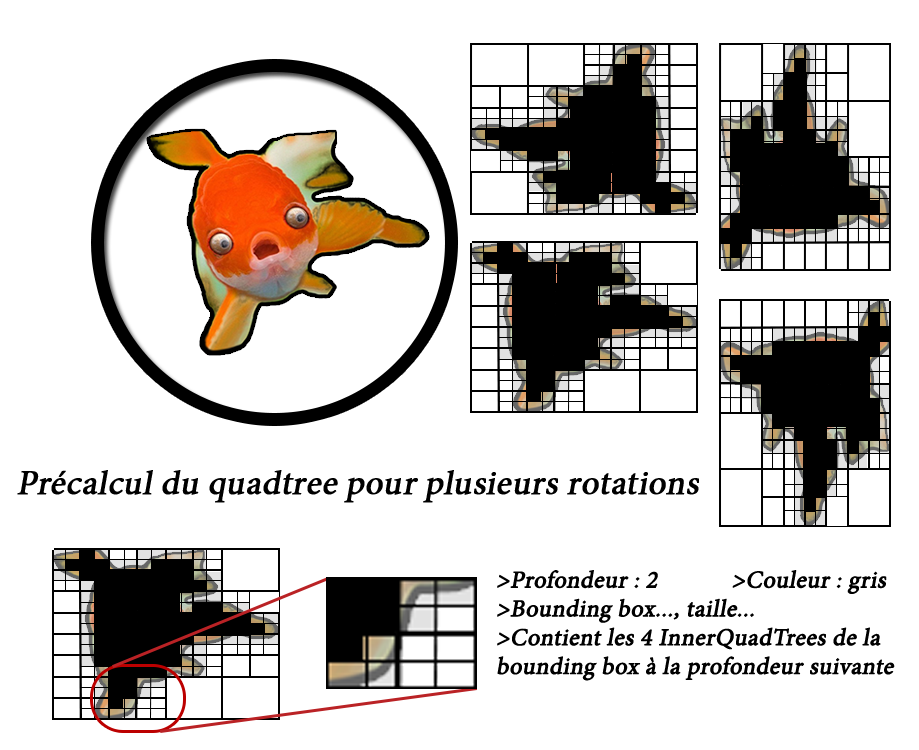
\includegraphics[scale=0.5]{img/innerquadtree.png}
\caption{Les InnerQuadTrees et leurs informations}
    \label{fig:innerquadtree}
\end{figure}

Pour tester la couleur de son espace et créer les sous-espaces suivants, un InnerQuadTree possède des méthodes appelant celles des bitmaps, représentés également par une classe. Un bitmap est une classe représentant un tableau de booléens qui est le même pour toutes les classes (utilisation d'un pointeur), avec les informations nécessaires pour situer la sous-zone concernée dans l'espace (offsets, taille...). La classe bitmap possède les méthodes primaires d'intersection, de translation, de rotation, de création etc.


\subsection{Parallélisme}

Une autre possibilité pour améliorer l'efficacité générale du programme est d'exploiter les architectures multicoeur qui sont disponibles sur les machines récentes. Nous avons utilisé cette notion de parallélisme de deux façons:\\

\subsubsection{Parallélisation d'un algorithme} Au cours du projet, nous avons développé plusieurs solutions. Certaines d'entre elles effectuant un grand nombre d'opérations indépendantes (notamment le \texttt{Simple Transformer}), il est possible de répartir le calcul de ces opérations sur plusieurs processeurs afin d'accélérer l'exécution du programme. 

\subsubsection{Parallélisation de plusieurs algorithmes} Certains algorithmes ayant un comportement non déterministe, plusieurs exécutions d'un même algorithme vont conduire à des résultats différents.
Nous avons donc implémenté un \texttt{Solver} permettant d'effectuer plusieurs calculs de solutions non déterministes et de conserver seulement le meilleur résultat.


\subsection{Interpolation améliorée}

Dans le but d'améliorer la vitesse d'exécution des algorithmes nous avons mis en place une méthode d'interpolation visant à réduire au maximum le nombre de points, tout en minimisant l'erreur induite.\\ 

Ceci permet d'effectuer plus rapidement les calculs internes aux algorithmes fonctionnant directement sur les modèles basés sur les points (\texttt{Shape}) en plus de permettre un calcul plus rapide des \texttt{QuadTrees}.\\

Nous utilisons pour cela différentes propriétés des courbes de Bézier. Notamment le fait qu'une courbe de Bézier définie sur un intervalle restreint reste une courbe de Bézier, il est donc possible de découper récursivement les courbes et ce sans perte de précision.\\

Il a ensuite été nécessaire de déterminer une condition d'arrêt pour cet algorithme. Il nous a semblé naturel d'approximer la courbe par une droite lorsque celle-ci est suffisamment "plate".\\ Nous avons donc choisi d'approximer l'erreur générée par cette approximation par le maximum des distances des points de la courbe à la droite. \\%% MEH

Ceci permet en effet d'avoir une approximation relativement précise de l'écart minimal qu'il est possible de se permettre en représentation interne afin d'éviter les intersections en sortie. \\%% endMEH
Nous n'avons cependant pas été en mesure de calculer un majorant exact de l'erreur due à cette approximation. \\

\begin{figure}[!htb]
\centering
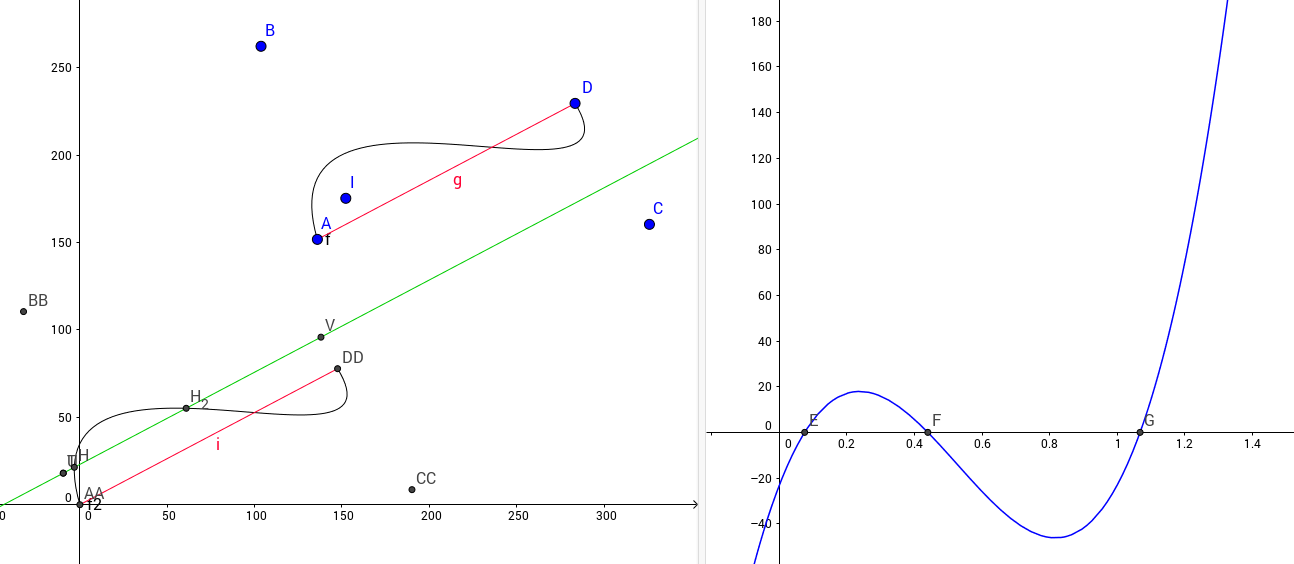
\includegraphics[scale=0.35]{img/BEZER.png}
\caption{Illustration de la recherche d'intersection}
\label{fig:rotos}
\end{figure}

Pour effectuer le calcul de cette distance maximale, nous calculons quatre points définissant les deux droites parallèles à celle définie par les deux points de contrôle de la courbe, qui se trouvent à une distance $d$ de celle-ci.\\

Nous utilisons ensuite la représentation paramétrique de ces droites, et de la courbe pour calculer s'il y a ou non intersection avec la courbe en résolvant une équation polynomiale du troisième degré sur l'intervalle $[0,1]$. Puis nous déterminons par dichotomie la distance $d$ maximale pour laquelle il y a intersection avec la courbe.\\

On peut voir sur la figure~\ref{fig:rotos} un exemple de droite s'intersectant avec une courbe de Bézier, et le polynôme associé.\\

Afin de compenser l'erreur ainsi produite, nous appliquons ensuite un \textit{buffer} autour de la forme définie par ces points, qui permet d'assurer que les bords de la nouvelle forme se trouvent à une distance égale à au moins deux fois l'erreur autorisée par l'approximation.\\

La marge d'erreur est réglable à la compilation, et une plus grande marge implique un \textit{buffer} plus important. On peut constater en figure~\ref{fig:rotos2} un exemple d'approximation très exagéré, avec le \textit{buffer} ajouté.

\begin{figure}[!htb]
\centering
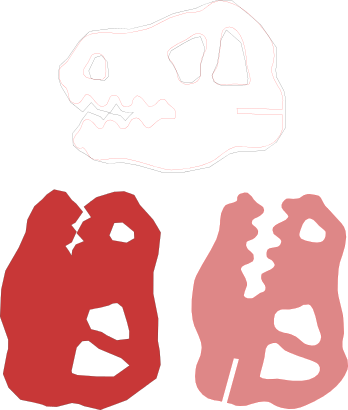
\includegraphics[scale=1.2]{img/approx.png} %non
\caption{Approximation (exagérée) d'une forme}
\label{fig:rotos2}
\end{figure}